\documentclass[11pt]{article}

\usepackage{booktabs}
\usepackage{graphicx}
\usepackage{listings}
\usepackage{amsfonts}
\usepackage{amsmath}
\usepackage{amssymb}
\usepackage{changepage}
\usepackage{hyperref}
\usepackage[margin=3cm]{geometry}

% meta
\title{Sistema di distribuzione logistica per Tribunali}
\author{Pietro Jomini}
\date{}

% document body
\begin{document}

% title
\pagenumbering{gobble}
\maketitle
\newpage
\tableofcontents
\newpage
\pagenumbering{arabic}

\section{Struttura dell'elaborato}
\subsection{Suddivisione in cartelle}

L'elaborato si suddivide nelle due cartelle principali ``Code'' e ``Docs''. La cartella ``Code'' contiene tutto il codice prodotto, mentre la cartella ``Docs'' contiene tutti i documenti scritti e i necessari schemi / immagini.

\subsection{Struttura del codice}

Il codice è diviso in cartelle per linguaggio di programmazione. La cartella ``python'' contiene l'implementazione dell'algoritmo MD5, la cartella ``sql'' lo script utilizzato per la creazione del database e le queries richieste, mentre la cartella ``web'' contiene l'applicazione web.

\subsection{Struttura di questo documento}

Le sezioni nel range $[2, 5]$ sono lo svolgimento della sezione 1 della traccia di svolgimento, mentre le sezioni dalla 6 sono in risposta alle sezioni successive.

\subsection{Schemi}

Gli schemi utilizzati sono stati realizzati tramite l'applicazione web \url{https://app.diagrams.net/} e renderizzati in png.

\newpage
\section{Infrastruttura di rete proposta}

Data la relativa semplicità e centralità del sistema si consiglia l'utilizzo di un servizio IAAS, ad esempio AWS EC2.

\section{Protocolli di rete utilizzati}

\subsection{HTTP}

HTTP is an application-level protocol and stands for ``HyperText Trasfer Protocol'', hinting that its main function is to tranfer hypertext documents.

\subsubsection{Use cases}

Hyptertext documents are text documents that arelinked togherer by links.The standard in the modern web is the HTML markup language, even tho nowadays is common to utilize high-level programming languages to build HTML documents, like ECMAScript(Javascript), Python or PHP.

Browsers are then responsible for rendering the desired hyptertex document in such a way that it is comprehensible to the end user, often enriching the experience with custom styles or scrips.

HTTP is commonly used for machine-to-user communications, but it's essential also in machine-to-machine situations. In those cases the preferred hypertex formats are JSON or XML.

\subsubsection{Communication}

HTTP follows the client-server model, where any number of client can request a document to a single server. Under the hoods it uses the TCP protocol, hence we know that two kind of connections are possible: ``persistent'' and ``not persistent'' ones.

\paragraph{Persistent connections}
When using a persistent connection the client and the server are connected for the whole communication process and can excange multiple files under the same connection. This is the preferred mode, since it reduces the total RTT.

\paragraph{Non persistent connections}
When using a non persistent connection the client and the server are connected only fot the time required to excange a single document. This solution is not preferred since it require a new TCP connection each time a document is excanged, increasing the total RTT.

\subsubsection{Header}

The HTTP header is divided in lines, separated by the escape characters ``cr lf'' (\textbackslash r\textbackslash n).
Each line is divided in fields by spaces.

\paragraph{First line}
The first line depends of the kind of message: the header be used both to send requests and responses. When sending a request the fields are ``method'', ``url'' and ``version''. When sending a response the fields are ``version'', ``status code'' and ``phrase''.

\paragraph{Header lines}
The followind $n$ lines, until a blank noe is met, forms the ``header lines''. Here each line hold a header value in the form ``Key: Value''. There is a large amount of ``header fields'', both standard and non standard, which fullfills a larga amount of tasks ranging from authentication to cookies.

\paragraph{Body}
Separated from the header lines by a blank line, the body contains the transferred payload, eg. the HTML content.

\paragraph{Method}
The first line of the HTTP request contains the field ``method''. This field tells to the server additional informations about the action that the client wants to perform on the requested file. The most used methods are:
\begin{center}
    \begin{tabular}{l|l}
        \toprule
        \textbf{Method} & \textbf{Description}                                     \\
        \midrule
        GET             & Retrieve the requested entity.                           \\
        HEAD            & Like a GET, but the server returns only the HTTP header. \\
        POST            & Send a new entity to the server.                         \\
        DELETE          & Delete an entity.                                        \\
        PATCH           & Modify an entity.                                        \\
        \bottomrule
    \end{tabular}
\end{center}
Those methods are heavily used when using the HTTP protocol for machine-to-machine comunications (eg. APIs).

\paragraph{Status}
The first line of the HTTP response contains the fields ``status code'' and ``phrase'' which serves the utility of communicating the status of the response. The field ``phrase'' contains the description of the given ``status code''. Status codes are divided in the following groups:
\begin{center}
    \begin{tabular}{l|l}
        \toprule
        \textbf{Code} & \textbf{Description} \\
        \midrule
        1**           & Informational        \\
        2**           & Succesfull           \\
        3**           & Redirects            \\
        4**           & Client errors        \\
        5**           & Server errors        \\
        \bottomrule
    \end{tabular}
\end{center}
which are specified furthermore by the last two digits. Some of thhe most common codes are:
\begin{center}
    \begin{tabular}{l|l}
        \toprule
        \textbf{Code}    & \textbf{Description}                                  \\
        \midrule
        200 OK           & The request has succeeded.                            \\
        301 MOVED        & The requested file has been moved.                    \\
        403 FORBIDDEN    & The client doesn't have access to the requested file. \\
        404 NOT FOUND    & The requested file hasn't been found.                 \\
        500 SERVER ERROR & Unhandled server error.                               \\
        \bottomrule
    \end{tabular}
\end{center}

\paragraph{418: I'm a teapot}
Defined as an april fool joke in the HTCPCP (HyperText Coffee Pot Control Protocol), indicates tha the server refues to brew coffe because it is, in fact, a teapot. Even tho it is considered a sort of ``easet egg'' in the HTTP protocol, it is sometime used as a repsonse to undesired requests, such as automated ones.

\subsection{SSH}

When connecting to our new EC2 virtual machine we use the SSH protocol. SSH stands for ``Secure SHell'' and, as the name mey hint, is used to safely connected to a remote command shell.

Under th hood it uses the TCP protocol and is divided in three internal protocols, which serves different purposes:

\paragraph{TLP}
The SSH Transport Layer Protocol implements server-side authentication.

\paragraph{UAP}
The SSH User Authentication Protocol implements client-size authentication.

\paragraph{CP}
The SSH Connection Protocol allows multiple channels to communicate over the same
encrypted tunnel.

\subsubsection{Encrypted tunnel}
SSH Creates encrypted tunnels (connections) where the communication between the two hosts is secure. Those are the steps it uses to do such:
\begin{enumerate}
    \item Both the server and clients have a public and private keys, used for an asymmetric cryptographic algorithm (eg. RSA).
    \item The client initiates the connection by contacting the server.
    \item The server sends to the client his public key.
    \item The client generate a random sequence of bits and sends it to the server, encrypted with the server's public key. The original string of bits is now used as the key for a symmetric cryptographic algorithm (eg. DES).
\end{enumerate}

\section{Sicurezza della infrastruttura di rete proposta}

\subsection{HTTPS}

\textit{Sebbene sia un protocollo di rete, quindi apaprtenente alla sezione 2, ho preferito descriverlo in questa sezione in quanto non è stato realmente utilizzato nella parte pratica dell'elaborato.}
\vspace{1em}

Il protocollo HTTP eredita dallo stack TCP/IP il problema della mancanza di sicurezza della connessione: essendo essa in chiaro, i messaggi sono intercettabili e modificabili. Per questo è solitamente usato il protocollo HTTPS (HTTP Secure) che combina il protocollo HTTP (approfondito alla sezione 3.1) con TTL.

\subsubsection{TTL}

Il protocollo TTL (Transport Layer Security) è un protocollo che si pone tra il livello di trasporto e il livello applicazione nello stack TCP/IP.

È internamente diviso in due protocolli:

\paragraph{Handshake}
Il protocollo di handshake gestisce la fase di negoziazione in cui il client e il server decidono l'algoritmo di cifratura e quello di scambio delle chiavi. Dopo la negoziazione il client e il server procedono allo scambio delle chiavi. Viene usato un'algoritmo simmetrico per la cifratura dei messaggi e uno asimmetrico per lo scambio della chiave simmetrica, ad esempio RSA (approfondito alla sezione 4.2).

\paragraph{Record protocol}
Il record protocol gestisce la cifratura dei messaggi secondo il seguente schema:
\begin{center}
    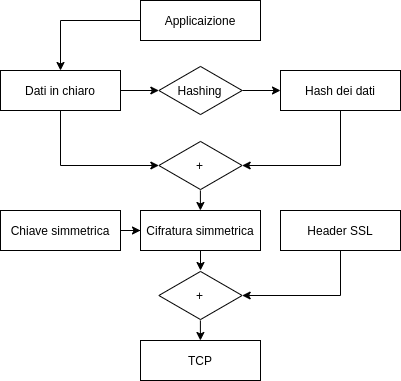
\includegraphics[scale=0.50]{./images/ttl.png}
\end{center}


\subsubsection{Certificati digitali}

Per certificare l'autenticità delle delle chiavi pubbliche scambiate in TTL vengono usati i certificati digitali.

I certificati digitali sono dei certificati rilasciati de un ente conosciuto, generalizzato come ``certificate authority'' (CA) atti a certificare la proprietà di un determinato file o dato.

In questo modo i client HTTPS possono verificare che le chiavi pubbliche scambiate tramite TTL siano di proprietà del server con il quale sono in fase di connessione.

\subsection{Privatezza degli endpoint}

\subsubsection{Sessione}

L'autenticazione dell'utente nella pagina web è permessa dalla presenza di una ``sessione'', che permette al server di avere dei dati mappati ad un client specifico.

Questo è a sua volta possibile grazie al cookies, dati che i client HTTP salvano per ogni dominio in modo che il dominio possa accedervi e modificarli. Il server salva dunque nei cookies del client una chiave che utilizza per indicizzare i dati che devono essere associati ad un client particolare.

In PHP (il linguaggio utilizzato per la codifica dell'applicazione web) la sessione si può utilizzare in questo modo:
\lstset{language=php}
\begin{lstlisting}
    // Inizializza la sessione e crea la
    // mappatura della chiave tra il server
    // e il client.
    session_start();

    // I dati salvati nella session sul server
    // sono ora accessibili nell'array $_SESSION
    $_SESSION['pi'] = 3.1415;
\end{lstlisting}

\subsubsection{Autenticazione}

L'utente è autenticato salvando il valore `Location', la chiave unica di due lettere che indica la posizione fisica del tribunale, nel campo `location' della sessione, che viene impostato durante il login.

Ogni volta che una pagina viene aperta viene controllato il campo e, se esso è vuoto, si redirige la request alla pagina di login: in questo modo le pagine diverse da quella di login sono inaccessibili ad ogni utente non autenticato.

\paragraph{Autenticità dell'utente}
Nella codificazione dell'applicazione web il controllo dell'autenticità dell'utente è permesso dalla presenza di una password, offuscata da un algoritmo di hashing (vedi sezione 4.1). In una produzione finalizzata ad un utilizzo reale sarebbe più sicuro avere della macchine, posizionate in ogni magazzino, che forniscono l'unico accesso al server tramite l'utilizzo di un firewall. Può essere implementata anche l'autenticazione della persona fisica che utilizza il servizio tramite una chiave digitale salvata su un supporto fisico.

\subsection{SQL injections}

È necessario prestare particolare attenzione ad ogni situazione in cui si costruisce dinamicamente una query SQL con dati richiesti in input all'utente.

Ad esempio, consideriamo la seguente interrogazione SQL:
\lstset{language=sql}
\begin{lstlisting}
    INSERT INTO
        Report(Box, Place, Date) 
    VALUES 
        ('$box','$place', '$date')
\end{lstlisting}
costruita per aggiungere un record alla tabella `Report'. I campi `\textdollar place', e `\textdollar date' sono richiesti in input all'utente: esso li inserisce tramite una forma HTML che esegue una richiesta HTTP di tipo POST all'endpoint dell'api designato alla creazione di nuovi elementi `Report'. Il campo `\textdollar box' è invece ottenuto tramite un parametro nell'URI impostato automaticamente.

Immaginando ora che l'utente inserisca nel campo `\textdollar place' la stringa
\begin{verbatim}
    a', '2021-05-30'); DROP TABLE Report;
\end{verbatim}
la query risultante sarà:
\lstset{language=sql, showstringspaces=false}
\begin{lstlisting}
    INSERT INTO
        Report(Box, Place, Date) 
    VALUES 
        ('$box','a', '2021-05-30'); 
    DROP TABLE Report;
        ', '$date')
\end{lstlisting}

La query costruita con la stringa inserita dall'utente con obiettivi malevoli ha il disastroso effetto di eliminare completamente la table `Report'. L'ultima riga della query inserita genera errore, ma la maggior parde dei server SQL eseguono comunque il codice precedente all'errore, e in caso contrario è facile immaginare come inserire una stringa che non generi errori.

Per evitare attacchi di questo tipo è necessario trattare i dati ottenuti in input dall'utente con la dovuta cura, ad esempio controllando che non contengano stringhe malevole. In PHP cioò può essere fatto utilizzando la classe PDO:
\lstset{language=php}
\begin{lstlisting}
    // Preparazione della query SQL
    $stmt = $connection->prepare("
        INSERT INTO Report(Box, Place, Date)
        VALUES (:box, :place, :date)
    ");

    // Inserimento dei valori in modo controllato
    $stmt->bindParam(':box', $box);
    $stmt->bindParam(':place', $place);
    $stmt->bindParam(':date', $date);    
\end{lstlisting}

\section{Utilizzo delle funzioni di hash oppure degli algoritmi crittografici}

\subsection{Hash}

Le funzioni di hash sono determinati algoritmi con le seguenti proprietà:

\paragraph{Generano digest di dimensione fissa}
Dato un messaggo $a$ di dimensione $k$ deve essere vera l'equazione $size(h(a)) = P$, dove $P$ è un valore predefinito.

\paragraph{Generano digest unici}
Dati due messaggi $a$ e $b$ deve essere vera l'equazione $h(a) \neq h(b)$, per qualsiasi $a$ e $b$. Questo è impossibile quando la dimensione predefinita del digest $P$ (vedi paragrafo precedente) è minore della dimensione dell'input, quindi l'obiettivo diventa di minimizzare le collisioni tra diversi input.

\paragraph{Generano digest irreversibili}
Dato un messaggo $a$, sconosciuto, deve essere difficile (se non impossibile) ricavarlo dal risultato della funzione $h(a)$.

\subsubsection{Esempio di implementazione}

\small{L'implementazione completa, scritta in linguaggio Python, è disponibile nella cartella ``code/python''.}

\paragraph{MD5}
MD5 è un algoritmo di hashing non sicuro: è stato infatti violato e con un computer moderno si può trovare una collisione in pochi secondi. La sua semplicità permette però di capirne il funzionamento in modo approfondito: questo è utile, dal momento che la maggior parte degli algoritmi più sicuri (eg. SHA2) si basano sugli stessi concetti.

L'algoritmo è diviso in tre fasi:

\paragraph{Padding}
In questa fase si corregge la dimensione dell'input, in modo che essa sia un multiplo di 512 bits.
\lstset{language=python}
\begin{lstlisting}
    # `message' is a bytearray
    # calculate the lenght of the message in bits
    L = len(message) * 8

    # if the message is longer than 2 ** 64,
    # we ``cut'' it to fit the maximum lenght.
    L &= 2 ** 64 - 1

    # find the number N such that L <= K * 512
    N = max((L - 1), 0) // 512 + 1
\end{lstlisting}
I bits mancanti sono riempiti da un `1', seguito da una serie di `0' fino ad arrivare al bit $N * 512 - 64$. Gli ultimi 64 bits sono riservati al contenimento di $L$.
\begin{lstlisting}
    # since we are using a bytearray,
    # we needs to scale down P to the
    # byte scale
    P //= 8

    # apply `1' and `0's padding
    message += bytearray([0x80] * min(P, 1) + [0x0] * (P - 1))

    # apply L padding
    # we can use python's native function `to_bytes'
    # which transforms an integer into a bytearray.
    # the byteorder parameters change the endian:
    #   a little-endian system stores the MSB at the location 
    #   with the smallest memory address (eg. to the right),
    #   while a big-endian system does the opposite
    message += L.to_bytes(8, byteorder="little")
\end{lstlisting}


\paragraph{Merging} In questa fase avviene la ``confusione'' dei dati in input. Dopo averli divisi in chunks da 512 bit, per ognuno di essi si applica in 64 iterazioni, numerate da 0 a 63, il seguente schema:
\begin{center}
    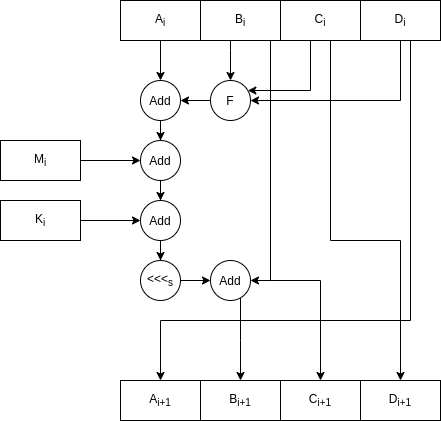
\includegraphics[scale=0.50]{./images/md5.png}
\end{center}.
La funzione F per l'iterazione i è così definita:
\begin{equation*}
    F(B, C, D) = \left\{
    \begin{array}{ll}
        (B \land  C) \lor (\lnot B \land D) & \lfloor \frac{i}{16} \rfloor = 0 \\
        (D \land  B) \lor (\lnot D \land C) & \lfloor \frac{i}{16} \rfloor = 1 \\
        B \oplus   C \oplus D               & \lfloor \frac{i}{16} \rfloor = 2 \\
        C \oplus (B \lor \lnot D)           & \lfloor \frac{i}{16} \rfloor = 3
    \end{array}
    \right.
\end{equation*}
mentre A, B, C, e D sono chiamati ``hash pieces'' e sono inizializzati con dei valori predefiniti per la prima iterazione. I valori costanti K sono dati dalla seguente funzione:
$$
    K(i) = \lfloor 2^{32} * \left\lvert sin(i + 1) \right\rvert  \rfloor
$$
e possono essere calcolati in anticipo, in modo da ridurre il tempo di elaborazione del digest. I valori M derivano invece dalla division in parole di 32 bit di dimensione del chunk corrente.

La funzione ``left-shift'' ($\lll_s$) è definita come:
$$
    \lll(F, s_a) = (F \ll s_a) \lor (F \gg (32 - s_a))
$$
\begin{equation*}
    a =  \left\{
    \begin{array}{ll}
        i                 & \lfloor \frac{i}{16} \rfloor = 0 \\
        (5i + 1) \bmod 16 & \lfloor \frac{i}{16} \rfloor = 1 \\
        (3i + 5) \bmod 16 & \lfloor \frac{i}{16} \rfloor = 2 \\
        7i \bmod 16       & \lfloor \frac{i}{16} \rfloor = 3
    \end{array}
    \right.
\end{equation*}
dove $s$ è una tabella di rotazione predefinita (consultabile nel file ``code/python/s.txt'').

\paragraph{Digest}
La creazione del digest avviene, dopo il completamente delle 64 iterazioni per tutti i chunk di dati, concatenando gli ``hash pieces'' A, B, C, e D risultanti. Si ottiene così un numero intero di dimensione 128 bit.

\paragraph{Digest esadecimale}
È comune utilizzare i digest sotto forma esadecimale. In python la conversione è semplice:
\begin{lstlisting}
    def hex_digest(digest: int) -> str:
    """Represent a md5 digest in hex format"""

        # the digest needs to be transformed from
        # little to big endian
        digest = digest.to_bytes(16, byteorder="little")
        digest = int.from_bytes(digest, byteorder="big")

        return "{:032x}".format(digest)
\end{lstlisting}

\subsubsection{Applicazioni pratiche}

Come già specificato nella sezione precedente, MD5 è ormai obsoleto per quanto riguarda la difficoltà nel trovare collisioni. A scopo didattico può essere comunque implementato nell'applicazione web: viene utilizzato per salvare sul database solo gli hash delle password, in modo da limitare il danno causato da un eventuale leak di dati (eg. a causa di una SQL injection).

È necessario un modo per eseguire il codice scritto in linguaggio python da un programma scritto in linguaggio PHP. Possiamo usare la funzione ``popen'':
\lstset{language=php}
\begin{lstlisting}
    $message = "The red frog and the blue bees";

    # open a file representing the standard 
    # output of the given command
    $cmd = "python ../python/md5.py '$message'";
    $stdout = popen($cmd, 'r');
    
    # read the first 32 charachters of the output,
    # which contains the digest
    $digest = fread($stdout, 32);

    # close the connection to the stdout file
    fclose($stdout);

    echo $digest; # a3346e9a6e65fe6ab88e41464e78b78b
\end{lstlisting}

Si crea dunque la funzione ``md5\_digest'' (la funzione ``md5'' è nativa in PHP) e si modifica il codice del login in modo da confrontare il digest della password inserita dall'utente con il valore salvato nel database.

\paragraph{Accesso indesiderato alla macchina}
La prima impressione che questo codice dovrebbe fare è di essere incredibilmente poco sicuro. Sembra prono ad attacchi simili alle injection SQL, in cui l'utente può eseguire comandi sul server in modo non autorizzato inserendo nel campo ``password'' stringhe come
\begin{verbatim}
    ' && rm -rf / && echo '
\end{verbatim}

Fortunatamente gli sviluppatori del linguaggio PHP hanno considerato questa debolezza e hanno implementato una funzione di sanificazione degli input. Inoltre, senza conoscere la password di amministratore del server (che renderebbe un attacco di questo tipo superfluo) è impossibile accedere in alcun modo a file a cui l'utente che esegue il codice PHP non ha accesso.

\section{Progettazione del database}
\subsection{Schema ER}

\begin{adjustwidth}{-5cm}{-5cm}
    \vspace{\fill}
    \begin{center}
        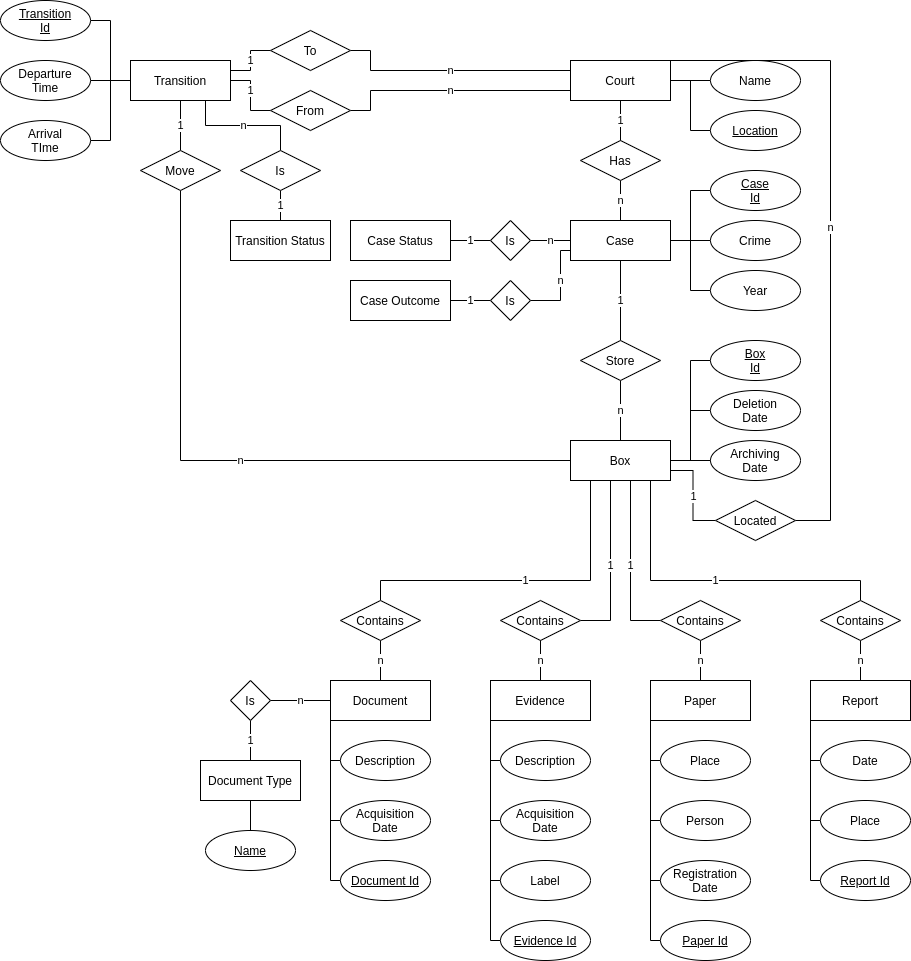
\includegraphics[scale=0.50]{./images/er.png}
    \end{center}
    \vspace{\fill}
\end{adjustwidth}

\subsection{Ipotesi}

\begin{itemize}
    \item Non possono essere eliminati elementi singoli all'interno di una scatola, ma è necessario eliminare l'intera scatola.
\end{itemize}

\subsection{Mapping}

Court(\underline{Location}, name, password) \\
Case(\underline{CaseId}, \textit{Court}, \textit{Status}, \textit{Outcome}, Crime, Year) \\
CaseStatus(\underline{Name}, Description) \\
CaseOutcome(\underline{Name}, Description) \\
Box(\underline{BoxId}, \textit{Case}, \textit{Location}, ArchivingDate, DeletionDate)

\noindent \\
Evidence(\underline{EvidenceId}, \textit{Box}, Description, AcquisitionDate, Label) \\
Paper(\underline{PaperId}, \textit{Box}, Place, PersonCF, RegistrationDate) \\
Report(\underline{ReportId}, \textit{Box}, Place, Date) \\
Document(\underline{DocumentId}, \textit{Box}, \textit{Type}, Description, AcquisitionDate) \\
DocumentType({\underline{Name})

\noindent \\
Transition(\underline{TransitionId}, \textit{Box}, \textit{From}, \textit{To}, \textit{Status}, DepartureTime, ArrivalTime) \\
TransitionStatus(\underline{Name}, Description)

\subsection{Normalizzazione}

\subsubsection{Prima forma normale}

Tutte le tabelle sono in prima forma normale, in quanto tutti i campi sono in forma atomica e ogni tabella ha una chiave primaria definita.

\subsubsection{Seconda forma normale}

Tutte le tabelle sono in seconda forma normale, in quanto non esistono campi non chiave che dipendono da una porzione di una chiave candidata composta.

\subsubsection{Terza forma normale}

Tutte le tabelle sono in terza forma normale, in quanto non esistono campi non chiave che dipendono da campi non chiave

\subsubsection{Forma normale di Boyce-Codd}

Tutte le tabelle sono nella forma normale di Boyce-Codd, in quanto tutti i campi determinanti sono superchiavi.

\subsection{Tabelle enumerabili}

Alcune tabelle hanno dei valori fissi ed enumerabili:

\subsubsection{Transition status}
\begin{center}
    \begin{tabular}{c|l}
        \toprule
        \textbf{Value} &
        \textbf{Description}                                           \\
        \midrule
        Requested      & The destintion court requested the transition \\
        Accepted       & The origin court accepted the transition      \\
        Transiting     & The transition is taking place                \\
        Completed      & The transition is completed                   \\
        \bottomrule
    \end{tabular}
\end{center}

\subsubsection{Case status}
\begin{center}
    \begin{tabular}{c|l}
        \toprule
        \textbf{Value} &
        \textbf{Description}                                    \\
        \midrule
        Preliminary    & Preliminary stage                      \\
        First          & Takes place before the court           \\
        Second         & Takes place before the court of appeal \\
        Third          & Takes place in cassation               \\
        Canceled       & The case is no longer active           \\
        \bottomrule
    \end{tabular}
\end{center}

\subsubsection{Case outcome}
\begin{center}
    \begin{tabular}{c|l}
        \toprule
        \textbf{Value} &
        \textbf{Description}                            \\
        \midrule
        Condemned      & The accused has been condamned \\
        Acquitted      & The accused has been aquitted  \\
        \bottomrule
    \end{tabular}
\end{center}

\section{Creazione del database}

Per la creazione del database è stato riportato il mapping in inguaggio SQL. La mappatura completa può essere consultata nel file ``code/sql/db.sql'', mentre sotto è riportato un esempio.

\subsection{Tabella di esempio}

Segue l'implementazione commentata della creazione della tabella ``Box'' in linguaggio SQL per il server MySQL:
\begin{lstlisting}[language=sql]
    CREATE TABLE 'Box' (
        -- inserimento dei campi
        'BoxId' int(11) NOT NULL AUTO_INCREMENT,
        'CaseT' int(11) NOT NULL,
        'Location' varchar(2) NOT NULL,
        'ArchivingDate' date NOT NULL,
        'DeletionDate' date DEFAULT NULL,
        'DeletionReport' TEXT DEFAULT NULL,

        -- keys
        PRIMARY KEY ('BoxId'),
        FOREIGN KEY ('CaseT') REFERENCES 'CaseT' ('CaseId'),
        FOREIGN KEY ('Location') REFERENCES 'Court' ('Location'),

        -- checks
        CHECK (
            'DeletionDate' IS NULL 
            OR YEAR('DeletionDate') - YEAR('ArchivingDate') >= 50
        ),
        CHECK (
            'DeletionDate' IS NULL 
            OR 'DeletionReport' IS NOT NULL
        )
    );
\end{lstlisting}

\subsubsection{Inserimento di dati}

Durante la creazione delle tabelle enumerabili (vedi sezione 6.5) è stata implementato anche l'inserimento dei valori possibili. Segue l'esempio della tabella ``TransitionStatus'':
\begin{lstlisting}[language=sql]
    INSERT INTO 'TransitionStatus' ('Name', 'Description') VALUES
        ('Accepted', 'The destintion court requested the transition'),
        ('Completed', 'The origin court accepted the transition'),
        ('Requested', 'The transition is taking place'),
        ('Transiting', 'The transition is completed');
\end{lstlisting}

\section{Queries aggiuntive}

Le tre queries aggiuntive sono consultabili nella cartella ``code/sql/queries''. La query 3 non può essere eseguita con un'interrogazione sola, ma è possibile ottentere il risultato desiderato con 4 interrogazioni separate.

\section{Applicazione WEB}

Il codice dell'applicazione WEB è consultabile nella cartella ``code/web''.

\subsection{Login}

Per autenticare il login è necessario inserire una password, della quale solo il digest MD5 è salvato nel database. Le password di default sono uguali alla locazione del tribunale: ad esempio, la password del tribunale di CN (Cuneo) è `CN'.

\subsection{Funzioni mancanti}

I link che richiedono funzioni non implementate redirigono ad una pagina che indica chiaramente lo stato di ``lavori in corso''. Alcune features sono mancanti ma non indicate da nessun link specifico:

\paragraph{Modifica dei casi}
Manca la possibilità di modificare i campi, che permetterebbe di fare uso dei campi ``status'' e ``outcome''.

\paragraph{Informazioni aggiuntive}
Al contrario che per gli items, non è al momento possibile vedere informazioni agginutive sui casi e sulle scatole.

\paragraph{Sanificazione delle queries SQL}
Non è stata implementata una corretta sanificazinoe delle queries SQL (pratica approfondita alla sezione 4.3).

\paragraph{Lifecycle delle transazioni}
Le transazioni hanno un lifecycle definito dal seguente schema:
\begin{center}
    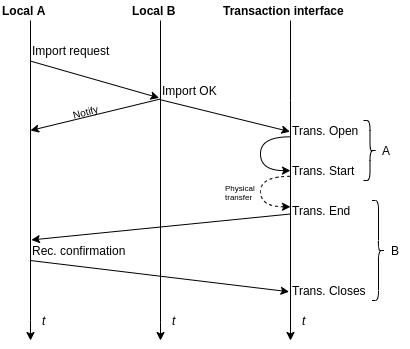
\includegraphics[scale=0.8]{images/tl.png}
\end{center}
ma non è stato implementata l'interfaccia per la notifica dell'inizio e fine del trasporto fisico, quindi lo stato della transazione salta l'inizio e la fine per diventare direttamente completato una volta accettato dal tribunale B:
\begin{center}
    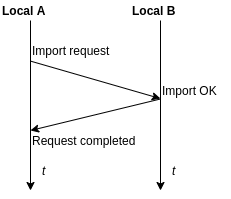
\includegraphics[scale=0.8]{images/tl1.png}
\end{center}

Manca anche la possibilità di negare un trasferimento: al momento l'unica opzione, nel caso non lo si desideri accettare, è lasciarlo in stato di richiesta.

\subsection{Grafica}
L'aspetto grafico è stato curato con HTML e CSS personalizzato, consultabile nella cartella ``code/web/css''.

\subsection{Paginazione}
Per poter implementare un sistema di paginazione che permettesse la non ripetizione del codice è stato necessario dividere il programma monolitico PHP in diverse pagine (nella cartella ``code/web/partials'') che sono renderizzate dallo spezzone di codice:
\begin{lstlisting}[language=php]
    $pages = [ ... ];
    $page = $_GET['page'];
    if ( in_array($page, $pages))
        require('../partials/' . $_GET['page'] . '.php');
\end{lstlisting}
che permette di indicare la pagina desiderata tramite il parametro URI ``page'' (eg. ?page=local) e, se la pagina richiesta è presente nella lista di pagine atorizzate, viene renderizzata. Ciò permette inoltre ai browser moderni di applicare solo le nuove modifiche alla pagina HTML, velocizzando il caricamente e rendendo l'esperienza per l'utente più piacevole.

È necessario il controllo sulle pagine autorizzate in modo che l'utente non possa accedere a files arbitari sul disco.

\end{document}